% !TEX TS-program = XeLaTeX
% use the following command: 
% all document files must be coded in UTF-8
\documentclass{textolivre}
% for anonymous submission
%\documentclass[anonymous]{textolivre}
% to create HTML use 
%\documentclass{textolivre-html}
% See more information on the repository: https://github.com/leolca/textolivre

% Metadata
\begin{filecontents*}[overwrite]{article.xmpdata}
    \Title{SEM model for technological, ecological and inclusive teacher training in times of pandemic}
    \Author{Antonio Hernández Fernández \sep Claudia de Barros Camargo}
    \Language{en}
    \Keywords{Teacher training \sep Technology \sep Inclusive education \sep Ecology \sep Covid-19}
    \Journaltitle{Texto Livre}
    \Journalnumber{1983-3652}
    \Volume{14}
    \Issue{2}
    \Firstpage{1}
    \Lastpage{13}
    \Doi{10.35699/1983-3652.2021.33640}

    \setRGBcolorprofile{sRGB_IEC61966-2-1_black_scaled.icc}
            {sRGB_IEC61966-2-1_black_scaled}
            {sRGB IEC61966 v2.1 with black scaling}
            {http://www.color.org}
\end{filecontents*}

% used to create dummy text for the template file
\definecolor{dark-gray}{gray}{0.35} % color used to display dummy texts
\usepackage{lipsum}
\SetLipsumParListSurrounders{\colorlet{oldcolor}{.}\color{dark-gray}}{\color{oldcolor}}

% used here only to provide the XeLaTeX and BibTeX logos
\usepackage{hologo}

% used in this example to provide source code environment
%\crefname{lstlisting}{lista}{listas}
%\Crefname{lstlisting}{Lista}{Listas}
%\usepackage{listings}
%\renewcommand\lstlistingname{Lista}
%\lstset{language=bash,
        breaklines=true,
        basicstyle=\linespread{1}\small\ttfamily,
        numbers=none,xleftmargin=0.5cm,
        frame=none,
        framexleftmargin=0.5em,
        framexrightmargin=0.5em,
        showstringspaces=false,
        upquote=true,
        commentstyle=\color{gray},
        literate=%
           {á}{{\'a}}1 {é}{{\'e}}1 {í}{{\'i}}1 {ó}{{\'o}}1 {ú}{{\'u}}1 
           {à}{{\`a}}1 {è}{{\`e}}1 {ì}{{\`i}}1 {ò}{{\`o}}1 {ù}{{\`u}}1
           {ã}{{\~a}}1 {ẽ}{{\~e}}1 {ĩ}{{\~i}}1 {õ}{{\~o}}1 {ũ}{{\~u}}1
           {â}{{\^a}}1 {ê}{{\^e}}1 {î}{{\^i}}1 {ô}{{\^o}}1 {û}{{\^u}}1
           {ä}{{\"a}}1 {ë}{{\"e}}1 {ï}{{\"i}}1 {ö}{{\"o}}1 {ü}{{\"u}}1
           {Á}{{\'A}}1 {É}{{\'E}}1 {Í}{{\'I}}1 {Ó}{{\'O}}1 {Ú}{{\'U}}1
           {À}{{\`A}}1 {È}{{\`E}}1 {Ì}{{\`I}}1 {Ò}{{\`O}}1 {Ù}{{\`U}}1
           {Ã}{{\~A}}1 {Ẽ}{{\~E}}1 {Ũ}{{\~u}}1 {Õ}{{\~O}}1 {Ũ}{{\~U}}1
           {Â}{{\^A}}1 {Ê}{{\^E}}1 {Î}{{\^I}}1 {Ô}{{\^O}}1 {Û}{{\^U}}1
           {Ä}{{\"A}}1 {Ë}{{\"E}}1 {Ï}{{\"I}}1 {Ö}{{\"O}}1 {Ü}{{\"U}}1
           {ç}{{\c{c}}}1 {Ç}{{\c{C}}}1
}


\journalname{Texto Livre}
\thevolume{14}
\thenumber{2}
\theyear{2021}
\receiveddate{\DTMdisplaydate{2020}{12}{11}{-1}} % YYYY MM DD
\accepteddate{\DTMdisplaydate{2021}{02}{28}{-1}}
\publisheddate{\today}
% Corresponding author
\corrauthor{Antonio Hernández Fernández}
% DOI
\articledoi{10.35699/1983-3652.2021.33640}
% list of available sesscions in the journal: articles, dossier, reports, essays, reviews, interviews, editorial
\articlesessionname{dossier}
% Abbreviated author list for the running footer
\runningauthor{Hernández Fernández and Camargo}
\editorname{Anna Izabella Miranda Pereira}

\title{SEM model for technological, ecological and inclusive teacher training in times of pandemic}
\othertitle{Modelo SEM para o treinamento tecnológico, ecológico e inclusivo de professores em tempos de pandemia}
% if there is a third language title, add here:
%\othertitle{Artikelvorlage zur Einreichung beim Texto Livre Journal}

\author[1]{Antonio Hernández Fernández \orcid{0000-0002-7807-4363} \thanks{Email: \url{antonio.hernandez@ujaen.es}}}
\author[2]{Claudia de Barros Camargo \orcid{0000-0002-2286-8674} \thanks{Email: \url{claudiadebarros@hotmail.es}}}

\affil[1]{Faculty of Humanities and Educational Sciences, Department of Pedagogy, Jaén, Spain.}
\affil[2]{Faculty of Education, Department of Education, Universidad Internacional Iberoamerica, Campeche, Mexico.}

\addbibresource{article.bib}
% use biber instead of bibtex
% $ biber tl-article-template

% set language of the article
\setdefaultlanguage{english}
\setotherlanguage[variant=brazilian]{portuguese}

% for spanish, use:
%\setdefaultlanguage{spanish}
%\gappto\captionsspanish{\renewcommand{\tablename}{Tabla}} % use 'Tabla' instead of 'Cuadro'
%\AfterEndPreamble{\crefname{table}{tabla}{tablas}}

% for languages that use special fonts, you must provide the typeface that will be used
% \setotherlanguage{arabic}
% \newfontfamily\arabicfont[Script=Arabic]{Amiri}
% \newfontfamily\arabicfontsf[Script=Arabic]{Amiri}
% \newfontfamily\arabicfonttt[Script=Arabic]{Amiri}
%
% in the article, to add arabic text use: \textlang{arabic}{ ... }

% to use emoticons in your manuscript
% https://stackoverflow.com/questions/190145/how-to-insert-emoticons-in-latex/57076064
% using font Symbola, which has full support
% the font may be downloaded at:
% https://dn-works.com/ufas/
% add to preamble:
% \newfontfamily\Symbola{Symbola}
% in the text use:
% {\Symbola }

% reference itens in a descriptive list using their labels instead of numbers
% insert the code below in the preambule:
\makeatletter
\let\orgdescriptionlabel\descriptionlabel
\renewcommand*{\descriptionlabel}[1]{%
  \let\orglabel\label
  \let\label\@gobble
  \phantomsection
  \edef\@currentlabel{#1\unskip}%
  \let\label\orglabel
  \orgdescriptionlabel{#1}%
}
\makeatother
%
% in your document, use as illustraded here:
%\begin{description}
%  \item[first\label{itm1}] this is only an example;
%  % ...  add more items
%\end{description}
 

% custom epigraph - BEGIN 
%%% https://tex.stackexchange.com/questions/193178/specific-epigraph-style
\usepackage{epigraph}
\renewcommand\textflush{flushright}
\makeatletter
\newlength\epitextskip
\pretocmd{\@epitext}{\em}{}{}
\apptocmd{\@epitext}{\em}{}{}
\patchcmd{\epigraph}{\@epitext{#1}\\}{\@epitext{#1}\\[\epitextskip]}{}{}
\makeatother
\setlength\epigraphrule{0pt}
\setlength\epitextskip{0.5ex}
\setlength\epigraphwidth{.7\textwidth}
% custom epigraph - END


% if you use multirows in a table, include the multirow package
\usepackage{multirow}

% add line numbers for submission
%\usepackage{lineno}
%\linenumbers

\begin{document}
\maketitle

\begin{polyabstract}
\begin{abstract}
This work tries to analyze the relationship between teacher training (TT), teacher training in inclusive education (TTIE), teacher training in technologies (TTT), teacher training in ecology (TTE) and teacher training in time of pandemic (TTP), through a confirmatory factor analysis (CFA) with structural equation model (SEM) of a Likert scale created \emph{ad hoc}, validated and confirmed. For the search for answers, a non-experimental, descriptive, explanatory and correlational research process has been carried out. The instrument used to collect the data has been a scale, which has been validated in content and with an excellent Cronbach's alpha (.902). The construct validity has been carried out with an exploratory factorial analysis (EFA). The sample has been of 598 students of Master's Degree in Teacher Training and the last year (4th) of the Primary Education Degree from the University of Jaen (Spain). It can be concluded that there is a relationship between the different forms of teacher training, from the correlational analysis the highest coefficient is between teacher training and teacher training in ecology and teacher training in inclusive education. From the CFA it is confirmed that this correlation is a very strong one, so that inclusion and ecology should be central axes in all teacher training, on the other hand, it concludes the low relationship between teacher training and teacher training in times of pandemic, so that, at least in theory, covid-19 should not affect teacher training.


\keywords{Teacher training \sep Technology \sep Inclusive education \sep Ecology \sep Covid-19}
\end{abstract}

\begin{portuguese}
\begin{abstract}
Este trabalho tenta analisar a relação entre treinamento de professores (TP), treinamento de professores em educação inclusiva (TPEI), treinamento de professores em tecnologias (TPT), treinamento de professores em ecologia (TPE) e treinamento de professores em tempo do pandemia (TPP), através de uma análise de fator de confirmação (AFC) com modelo de equação estrutural (SEM) de uma escala Likert criada \emph{ad hoc}, validada e confirmada. Para a busca de respostas, foi realizado um processo de pesquisa não-experimental, descritivo, explicativo e correlacional. O instrumento utilizado para coletar os dados foi uma escala,  validada em conteúdo e com um excelente alfa Cronbach (.902). A validade da construção foi realizada com uma análise fatorial exploratória (AFE). A amostra foi de 598 alunos de Mestrado em Formação de Professores e o último ano (4º) do Ensino Primário da Universidade de Jaen (Espanha). Pode-se concluir que existe uma relação entre as diferentes formas de formação de professores. A partir da análise correlacional, o maior coeficiente é entre formação de professores e formação de professores em ecologia e formação de professores em educação inclusiva. A partir da AFC confirma-se que essa correlação é uma relação muito forte, de modo que a inclusão e a ecologia devem ser eixos centrais em toda a formação de professores; por outro lado, conclui-se a baixa relação entre formação de professores e formação de professores em tempos de pandemia, de modo que, pelo menos em teoria, a Covid-19 não deve afetar a formação de professores.


\keywords{Treinamento de professores \sep Tecnologia \sep Educação inclusiva \sep Ecologia \sep Covid-19}
\end{abstract}
\end{portuguese}

% if there is another abstract, insert it here using the same scheme
\end{polyabstract}


\section{Introduction}\label{sec1intro}
At the end of 2019, in Wuhan City, a type of coronavirus, the 2019-nCoV, renamed SARS-CoV2 (covid19), which is causing social and educational changes. Training, both initial and continuous, has entered a process of adaptation and reinvention, adapting to the demands imposed by the pandemic, such as the increasing use of digital platforms for teaching in primary, secondary and higher education, as well as changes in traditional approaches to initial training in a university context, such as continuous training for teachers at any level and in any situation. This research adopts teacher training in its classic levels: initial and continuous, questioning the relationship that can be established between teacher training in inclusive education, ecological technology and training in times of pandemic, generating a research instrument to analyze this relationship.

\textcite{nieva2016}, %Nieva and Martínez (2016), 
consider teacher training as a key factor to transform a society that gives value to human development, which is why it is convenient to relate teacher training with personal training, theoretical and disciplinary training and research training, giving, in addition, great emphasis to the development of values such as freedom, respect, solidarity and other inclusive values \cite{diazquero2006}. %(DÍAZ QUERO, 2006). 
Another factor comes from the fact that teachers must be trained in the fields of knowledge, before exercising the teaching function \cite{aravena2020}, %(ARAVENA, 2021), 
it is not difficult at present to find teachers at the university level teaching practical disciplines without ever having exercised the profession, and thus agreeing with \textcite{rodriguez2021} %Rodríguez, Miqueli and Dávila (2021)
in the sense that the characteristics of the XXI century inevitably produce changes, so that a teaching staff with a high quality professional development is demanded. Teacher training is configured as a key element in society; however, social and educational changes will transform teacher training and the very social valuation of it; \textcite{vaillant2015}, %Vaillant and Marcelo, in 2015, 
already investigated on these processes of social and educational change, which now in pandemic are much more extreme.

By the other hand, according to \textcite{infante2011}, %Infante (2011), 
teacher training it is a challenge for educational centers, being also a way of redefining the concept of inclusion. Thus, it is necessary to provide training that responds to diversity from the perspective of inclusion, not only by knowing how to eliminate architectural barriers, but also by training in a critical analysis of the systems of inclusion and exclusion. Thus, teacher training in the field of inclusion is undergoing substantial changes in recent years, from the idea of \textcite{booth2000}, %Booth and Ainscow (2000), 
which emphasizes the idea of inclusion based on inclusive policies, inclusive practices and inclusive culture, to a more realistic vision based on the development of inclusive values as a starting point to achieve real inclusion \cite{arnaiz2019}. %(ARNAIZ, 2019).

It is impossible to foresee whether the "new normal" that has been imposed with the covid19 pandemic will lead to new confinements and greater restrictions, which will continue in very particular scenarios. Thus, students with specific educational support needs will continue to lose social contact, difficulties in developing and implementing curricular adaptations, the near impossibility of applying university design parameters for learning/instruction, etc., increasingly blurring integration, let alone inclusion \cite{moreno2020}. %(MORENO; TEJADA; DÍAZ, 2020). 
Therefore, it is not too bold to think that all this will affect teacher training for inclusion.

Technology has been another key element in the new pandemic scenario. \textcite{talavera2020} %Talavera and Junior (2020)
show the difficulties of the transition from a face-to-face context to a virtual teaching-learning scenario, proposing the teaching of appropriate behavior within the digital culture, as well as training teachers in virtual training methodologies and emotional accompaniment to students and their families. \textcite{dussel2020} %Dussel (2020) 
emphasizes the teaching work in the pandemic, so that we are witnessing a process of selection and hierarchization in the digital environment, and also many ways of carrying out teaching practices without necessarily being in the classroom as a physical space, and this is one of the great lessons learned in times of pandemic. Thus, socio-technical environments emerge as a conjunction of artifacts and technologies with human actions, as mutually intertwined entities. It is necessary to highlight some issues caused by covid19, thus, for example, in general, Latin countries have high shortcomings to ensure access and quality conditions in virtual education \textcite{sanchez2020}, %Sanchez, Quiroga and Ospina (2020), 
on the other hand, \textcite{tejedor2020} %Tejedor, Cervi, Tusa and Parola (2020) 
highlight the negative assessment of students about the transition to virtuality. Thus, the greatest challenge that the pandemic has caused in teacher training in technologies will be given by the renewal of methodological strategies in the teaching-learning process, i.e., it is not possible to apply a face-to-face methodology to a virtual reality, or we will be doomed to failure \cite{talavera2020}. %(TALAVERA; JUNIOR, 2020).
All of the above leads us to the cornerstone of all the changes that have taken place under the pandemic and which lie in the transformation of the training of university teachers \cite{suarez2020}, %(SUÁREZ, 2020),
either because they have to adapt to the current world, or because it is necessary to go towards a responsible re-contextualization according to the demands of today's society.

The research in this paper includes ecological teacher training as a variable to be taken into account, an issue that may seem out of context, but which is considered here as key in the training of a 21st century teacher. \textcite{bermudez2008} %Bermúdez and De Longhi (2008) 
detail the elements that constitute ecology and that would be key objects for teacher training, thus, we highlight evolution, nutrition, cell, ecosystem, natural environment, biodiversity, solidarity with living beings, tolerance with different species, etc. We hardly find studies on ecological teacher training, as a conceptually defined element, certainly, with the pandemic of covid19 the teacher cannot be alien to this training, where natural environments, biology, environment, living beings..., have taken an extreme relevance. We end with \textcite{esteve2009} %Esteve (2009) 
when he states that the profound processes of social change that have taken place in recent decades have posed new problems for teacher training, which we have not yet been able to assimilate. With the arrival of the coronavirus pandemic, it is evident that Esteve's words fall short of Esteve's words, given the dimension and profound impact that is being experienced under covid19.

\section{Method}\label{sec2method}
This research is based on the general objective: to analyze the relationship between teacher training, teacher training in educational, technological and ecological inclusion and teacher training in times of pandemic. The specific objectives are: 1.-To review theoretically the research topics; 2.-To validate the research instrument in content and construct; and, finally, 3.-To show the relationships between dimensions through CFA. The research design is non-experimental \cite{kerlinger1979}, %(KERLINGER, 1979), 
descriptive-explanatory \cite{arias2012} %(ARIAS, 2012) 
and correlational \cite{schuyler2008}, %(SCHUYLER, 2008), 
with a quantitative methodology \cite{hernandezsampieri2010}, %(HERNÁNDEZ SAMPIERI; FERNÁNDEZ; BAPTISTA, 2010),
and as a reference an interpretative paradigm \cite{perezserrano2004}. %(PÉREZ, 2004). 
In order to carry out the research, a Likert scale was chosen as the research instrument.

The sample drawn from students in their final year (4th) of the Primary Education Degree and those in the Master's Degree in Teacher Training at the University of Jaen. The entire population (600 subjects) was selected, which finally consisted of: 298 subjects in their 4th year and 300 subjects in the Master's Degree, for a total of 598 participants. The study population is justified because we want to take data from subjects who are finishing their studies as future teachers in primary education centers and compare them with subjects who finished their undergraduate studies and are in the master's degree of teacher training (where there are participants of various specialties) that qualifies them to be teachers in secondary education centers, thus covering a broad spectrum of the educational system, in addition to focusing on subjects in initial training and participants in postgraduate and continuing education.

The dimensions of this study, extracted from the theoretical framework are: A.-Teacher training (TT), B.-Teacher training in inclusive education (TTIE), C.-Teacher training in technologies (TTT), D.-Teacher training in ecology (TTE), and E.-Teacher training in pandemic time (TTP). The dependent variables are: inclusion, technology, ecology and pandemic, the independent variable is: training. The hypothesis established is: H0.-There is a relationship between inclusive, technological and ecological teacher training and teacher training in times of pandemic. The software used for the statistical study was SPSS v25 and Lisrel 8.80.

The instrument is a Likert scale with an odd number of options, five response levels and a range of 1 to 5, which was constructed with an operationalization table \Cref{tab1}. Five dimensions were established, with a total of 25 items.

%\begin{small}
%\renewcommand{\arraystretch}{1.5}
\begin{longtable}{p{0.2\textwidth}p{0.2\textwidth}p{0.2\textwidth}}
\caption{Operationalization table.}
\label{tab1}
\\ 
\toprule 
Dimensions & Variables & Items \\ 
\midrule
\arrayrulecolor[gray]{.7}
A. - TT. \newline \textcite{nieva2016} \newline \textcite{rodriguez2021} & Teacher training. & 
\multicolumn{1}{p{0.5\textwidth}}{A1. - Current teacher training satisfies my training needs. \newline
A2. - University teaching training is sufficient for my educational practice. \newline
A3. - The teacher training offered by non-university institutions is sufficient for my educational practice. \newline
A4. - Teaching training offered by foreign institutions is of higher quality than the national one. \newline
A5. - Teacher training is the key to an educational system in accordance with the 21st century.}
\\
\midrule
B. - TTIE. \newline \textcite{booth2000} \newline \textcite{arnaiz2019} \newline \textcite{moreno2020} & Teacher training in inclusive education. & \multicolumn{1}{p{0.5\textwidth}}{B6. - Current inclusive teacher training satisfies my training concerns. \newline
B7. - The inclusive teacher training offered by the university is sufficient for my educational practice. \newline
B8. - The inclusive teacher training offered by non-university institutions is sufficient for my educational practice. \newline
B9. - Inclusive teacher training offered by foreign institutions is of higher quality than the national one. \newline
B10. - Inclusive teacher training is the key to a 21st century education system.}
\\
\midrule
C. - TTT. \newline \textcite{talavera2020} \newline \textcite{dussel2020} \newline \textcite{suarez2020} & Teacher training in technologies. & \multicolumn{1}{p{0.5\textwidth}}{C11. - The current technological teacher training satisfies my training concerns. \newline
C12. - The technological teacher training offered by the university is sufficient for my educational practice. \newline
C13. - The technological teacher training offered by non-university institutions is sufficient for my educational practice. \newline
C14. - Technological teacher training offered by foreign institutions is of higher quality than the national one. \newline
C15. - Technological teacher training is the key to an educational system in line with the 21st century.}
\\
\midrule
D. - TTE. \newline \textcite{bermudez2008} & Teacher training in ecology. & 
\multicolumn{1}{p{0.5\textwidth}}{D16. - The current ecological teacher training satisfies my training concerns. \newline
D17. - The ecological teacher training offered by the university is sufficient for my educational practice. \newline
D18. - The ecological teacher training offered by non-university institutions is sufficient for my educational practice. \newline
D19. - Ecological teacher training offered by foreign institutions is of higher quality than the national one. \newline
D20. - Ecological teacher training is the key to a 21st century education system.}
\\
\midrule
E. - TTP. \newline \textcite{esteve2009} & Teacher training in times of pandemic. & 
\multicolumn{1}{p{0.5\textwidth}}{E21. - Current teacher training meets my training concerns in times of pandemic. \newline
E22. - The inclusive teacher training offered by the university is sufficient for my educational practice in times of pandemic. \newline
E23. - The technological teacher training offered by non-university institutions is sufficient for my educational practice in times of pandemic. \newline
E24. - Ecological teacher training offered by foreign institutions is of higher quality than the national one in times of pandemic. \newline
E25. - Teacher training is the key to an educational system in accordance with the XXI century in times of pandemic.}
\\
\arrayrulecolor{black}
\bottomrule
%\end{tabular}
\source{own elaboration.}
\centering
\end{longtable}
%\end{small}

\Cref{tab1} shows how the Likert scale was constructed, using the theoretical framework, dimensions and variables as a guide.

\section{Results}\label{sec3results}
Content validity was assessed by means of expert judgment and pilot testing. In relation to the expert judgment, the (a) expert competence coefficient, (b) content validity of the instrument, and (c) inter-observer agreement analysis was calculated. (a) K is obtained from the knowledge coefficient (Kc) and the argumentation coefficient (Ka), obtaining a value of .91, which is high \cite{blasco2010}. %(BLASCO; LÓPEZ; MENGUAL, 2010). 
(b) The content validity of the instrument was carried out using the Lawshe method (1975) modified by \textcite{tristan2008}, %Tristán (2008), 
which shows that the items as a whole are valid when reaching a global validity index (CVI) of .93. (c) The interobserver agreement analysis was carried out using the Fleiss kappa index, obtaining a result of .940 (Sig .000), which corresponds to an almost perfect agreement between experts \cite{landis1977}. %(LANDIS; KOCH, 1977). 
Finally, it can be concluded that the total content validity of the instrument is .96, or 92.6\%. On the other hand, the judges suggested minor changes in the wording of some items and aspects of syntactic concordance, which were resolved, so we can move on to the pilot test, which was conducted by administering the scale to a group of subjects drawn from the sample, subsequently applying face validity, in which it was concluded that 93\% of the subjects who participated in this phase expressed that the questionnaire was clear and accurate and 95\% that it was understandable.

The reliability of the scale was calculated according to the intercorrelation of items, this analysis is carried out through Cronbach's alpha, which in this case gives an excellent value (.902).

Construct validity was performed by means of the PFA following the following steps:

Preliminary analysis: the Kaiser-Meyer-Olkin measure of sampling adequacy (KMO coefficient) has been used, in our case the value is .778, following \textcite{kaiser1974} %Kaiser (1974)
the value is acceptable, the result of Bartlett's test of sphericity is .000 and the Determinant 1.299E-8, so we continue with the analysis.

\begin{table}[htpb]
\caption{KMO and Bartlett's test.}
\label{tab2}
\centering
\begin{tabular}{p{0.3\textwidth}p{0.2\textwidth}p{0.1\textwidth}}
\toprule 
\arrayrulecolor[gray]{.7}
\multicolumn{2}{c}{Kaiser-Meyer-Olkin Measure of Sampling Adequacy.} & ,778
\\ 
\midrule
\multirow{3}{*}{Bartlett's Test of Sphericity} & Approx. Chi-Square & 10511,117 \\
\cmidrule{2-3}
& df & 300 \\
\cmidrule{2-3}
& Sig. & ,000
\\
\arrayrulecolor{black}
\bottomrule
\end{tabular}
\source{own elaboration.}
\centering
\end{table}

\Cref{tab2} shows the Kaiser-Meyer-Olkin values, Bartlett's test of sphericity and the significance, which, being within the accepted terms, allows us to continue with the FEA.
 
Analysis of the structure of the correlations: the resulting table of communalities showed us that the factors have a value higher than .510, so it is not necessary to eliminate any item from the factor analysis. The best represented items are: E24 (.881).-Ecological teacher training offered by foreign institutions is of higher quality than the national one in times of pandemic.
E25(.832).-Teacher training is the key to an educational system in accordance with the 21st century in times of pandemic. The worst represented item is: E22 (.510).- E22.-Inclusive teacher training offered by the university is sufficient for my educational practice in times of pandemic. We then proceed to calculate the total variance explained to determine the corresponding factors (\Cref{tab3}).

\begin{table}[htpb]
\caption{Total variance explained.}
\label{tab3}
\centering
\begin{tabular}{p{0.12\textwidth}lllllll}
\toprule 
\multirow{2}{*}{Component} & \multicolumn{3}{c}{Initial Eigenvalues} & \multicolumn{3}{c}{Rotation Sums of Squared Loadings} \\ 
\cmidrule{2-4} \cmidrule{5-7}
& Total & \% of Variance & Cumulative \% & Total & \% of Variance & Cumulative \%
\\
\midrule
1 & 8,273 & 33,091 & 33,091 & 5,007 & 20,026 & 20,026 \\
2 & 2,606 & 10,425 & 43,516 & 3,061 & 12,243 & 32,269 \\
3 & 2,320 & 9,282 & 52,798 & 3,033 & 12,131 & 44,400 \\
4 & 2,122 & 8,486 & 61,284 & 2,992 & 11,968 & 56,368 \\
5 & 1,310 & 5,239 & 66,523 & 2,511 & 10,044 & 66,412 \\
6 & 1,126 & 4,504 & 71,027 & 1,154 & 4,615 & 71,027 \\
7 & ,920 & 3,679 & 74,705 & & & \\
\bottomrule
\end{tabular}
\source{own elaboration.}
\centering
\end{table}

\Cref{tab3} shows the factors and the corresponding variances, with the first seven factors explaining 74.705\% of the accumulated explained variance.

Determination of the model: the distribution of items according to the highest level of saturation by factors (greater than 3 items) is reduced to factor F1: A.-Teaching training (A1, A2, A3, A4, A5). B.-Inclusive teacher training (B6, B7, B8, B9, B10). C.-Technological teacher training (C11, C12, C13, C14). D.-Ecological teacher training (D16, D17, D18, D19, D20). E.-Teaching training in pandemic (E21, E22, E24, E25). We calculated Cronbach's alpha for factor 1 (.903) for 23 items, which gives an "excellent" rating (2-item reduction). Reliability is slightly higher than the original scale.

\subsection{Hypothesis testing.}\label{subhypotest}
The ANOVA of the different dimensions with the variable "degree/master's degree" was carried out by calculating Fisher's F (\Cref{tab4}), which shows that the relationship from highest to lowest is between the following:

Degree/Master and Dimension B (F=1.240), Degree/Master and Dimension C (F=0.911) and finally, Degree/Master, Dimension D (F=0.569), Dimension E (F=0.124) and Dimension A (F=0.028). The strongest relationship is between inclusive teacher training and followed by technological teacher training and Degree/Master, with difference from the rest of the dimensions.

\begin{table}[htpb]
\caption{ANOVA.}
\label{tab4}
\centering
\begin{tabular}{p{0.15\textwidth}lllllll}
\toprule 
& & Sum of Squares & df & Mean Square & F & Sig.
\\
\midrule
\arrayrulecolor[gray]{.7}
\multirow{3}{*}{TT} & Between Groups & 0,017 & 1 & 0,017 & 0,028 & 0,868 \\
& Within Groups & 366,763 & 596 & 0,615 & & \\
& Total & 366,780 & 597 & & & \\
\midrule
\multirow{3}{*}{TTIE} & Between Groups & 0,623 & 1 & 0,623 & 1,240 & 0,266 \\
& Within Groups & 299,541 & 596 0,503 & & \\
& Total & 300,165 & 597 & & & \\
\midrule
\multirow{3}{*}{TTT} & Between Groups & 0,517 & 1 & 0,517 & 0,911 & 0,340 \\
& Within Groups & 333,247 & 587 & 0,568 & & \\
& Total & 333,764 & 588 & & & \\
\midrule
\multirow{3}{*}{TTE} & Between Groups & 0,360 & 1 & 0,360 & 0,569 & 0,451 \\
& Within Groups & 376,914 & 596 & 0,632 & & \\
& Total & 377,274 & 597 & & & \\
\midrule
\multirow{3}{*}{TTP} & Between Groups & 0,062 & 1 & 0,062 & 0,124 & 0,725 \\
& Within Groups & 297,129 & 596 & 0,499 & & \\
& Total & 297,191 & 597 & & & \\
\bottomrule
\end{tabular}
\source{own elaboration.}
\centering
\end{table}

\Cref{tab4} shows two very interesting values in this research, on the one hand, the strength of the relationship between the dimension and the sample groups (the highest strength corresponds to dimension B and the lowest to dimension A) and, on the other hand, the level of significance to reject the null hypothesis of equality (p<.005), in this case, we accept the equality of the means, so there are no differences in responses to the items between the two groups.

\subsection{Correlation analysis.}\label{subcorreanaly}
To perform the correlation we used Pearson's correlation, since according to the Mann-Withey U test we have a normal distribution of data, with the highest values being the following: E24<>E25 (.790), A4>B9 (.730), B9>A4 (.730), B8>B7 (.727), D16<>D17 (.706), D18>D17 (.703) and C13>D18 (.702). By dimensions, the highest correlations are: DIM A<>>DIM B (.789) and DIM D>DIM B (.765). We developed the highest ones:

E24<>E25 (.790): E24.-Ecological teacher training offered by foreign institutions is of higher quality than national teacher training in times of pandemic. E25.-Teacher training is the key to a 21st century education system in times of pandemic.

TT<> TTIE (.789): Teacher training and inclusive teacher education. TTE> TTIE (.765). Ecological teacher education and inclusive teacher education.

\subsection{Descriptive analysis.}\label{subdescanaly}
With respect to the descriptive analysis, we will highlight, by dimensions, some of the responses of the research subjects that are relevant to appreciate the ideas of the sample group on the subject under investigation.

In Dimension A (TT), subjects generally respond "disagree" with its items (mean=2.90).

\begin{figure}[htbp]
 \centering
 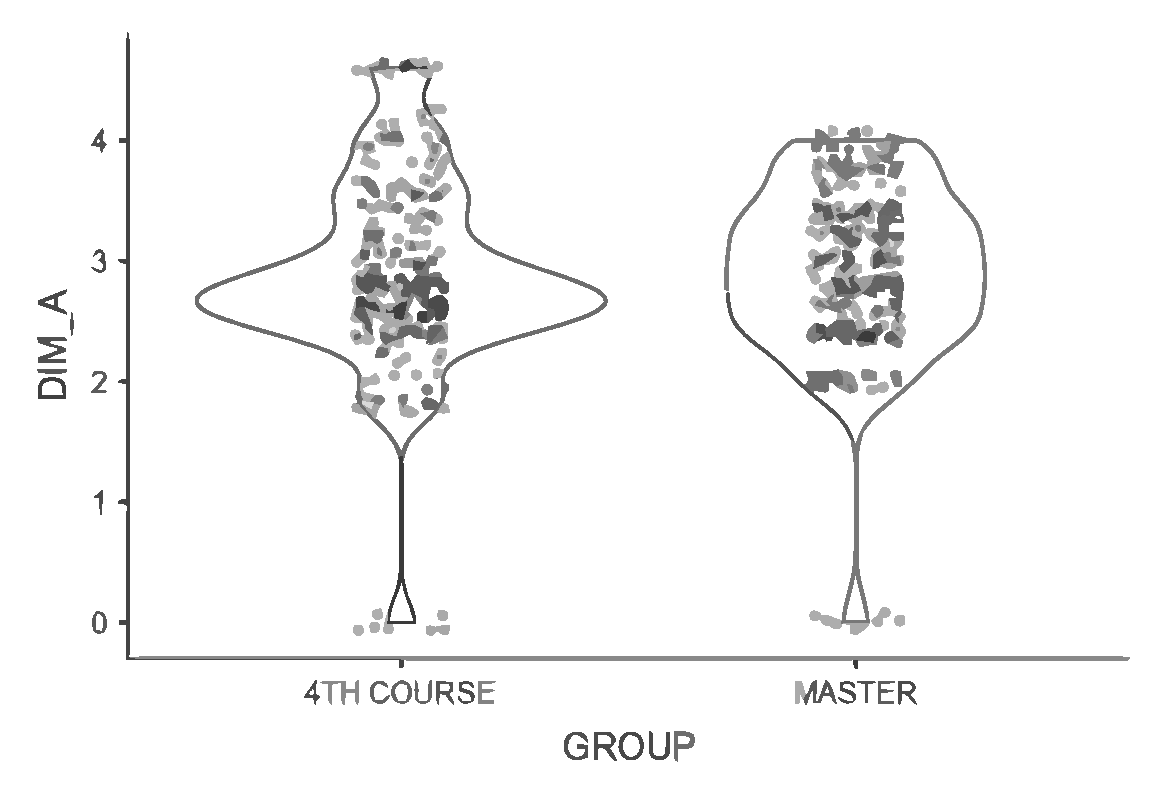
\includegraphics[width=0.65\textwidth]{fig1.pdf}
 \caption{Descriptive data for dimension A.}
 \label{fig1}
 \source{own elaboration.}
\end{figure}

\Cref{fig1} shows the grouping of responses in both the undergraduate and master's degree groups, we observe that there is similarity, with responses grouped around "disagree" and very close to indifferent.

In reference to dimension B (TTIE), the subjects are "indifferent" (mean=3.05) in their responses to the items of this dimension.

\begin{figure}[htbp]
 \centering
 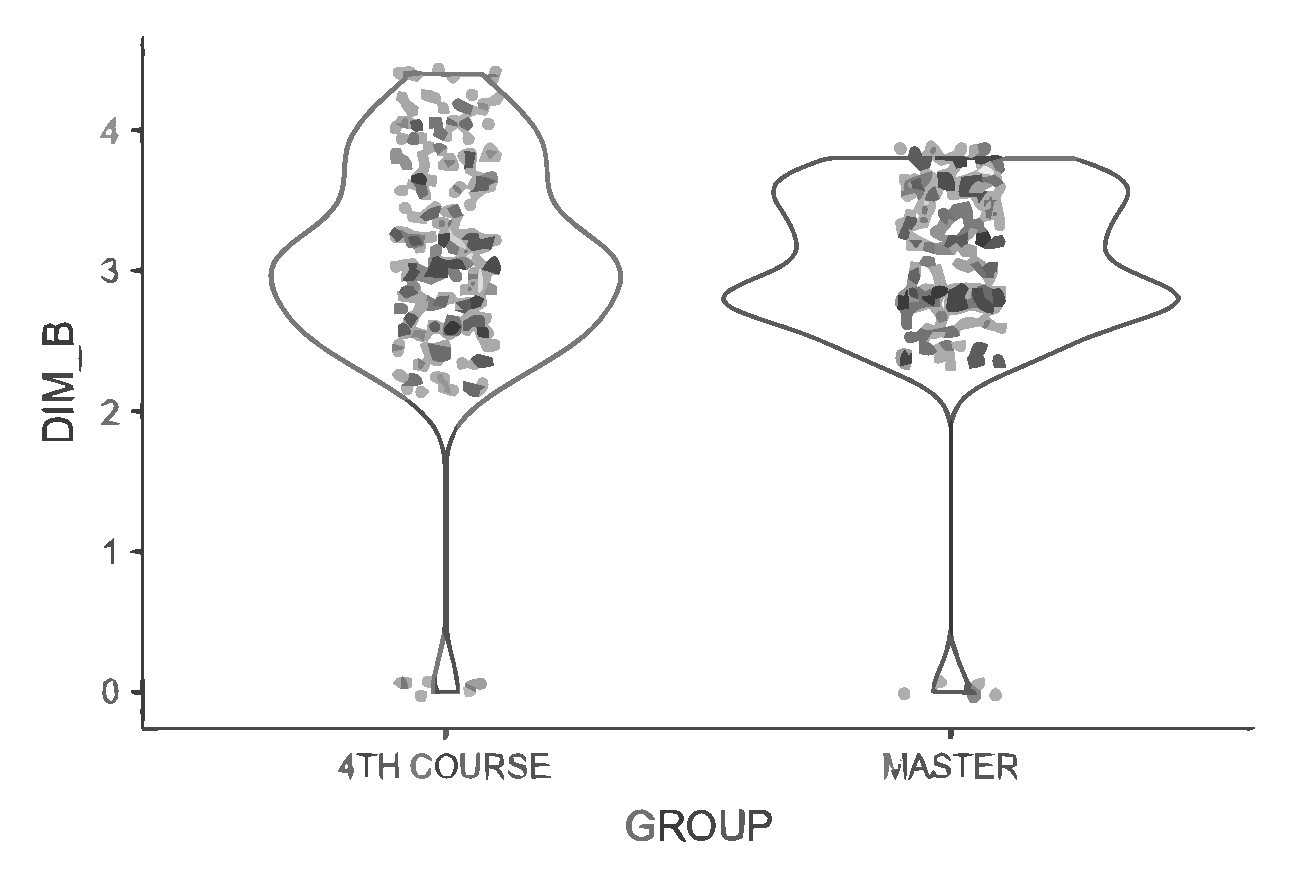
\includegraphics[width=0.65\textwidth]{fig2.pdf}
 \caption{Descriptive data for Dimension B.}
 \label{fig2}
 \source{own elaboration.}
\end{figure}

\Cref{fig2} shows the grouping of responses regarding inclusive teacher training, which is indifferent to the questions asked, with little difference between the two sample groups.

As for dimension C (TTT), the participants are indifferent to the questions in this dimension (mean=3.054).

\begin{figure}[htbp]
 \centering
 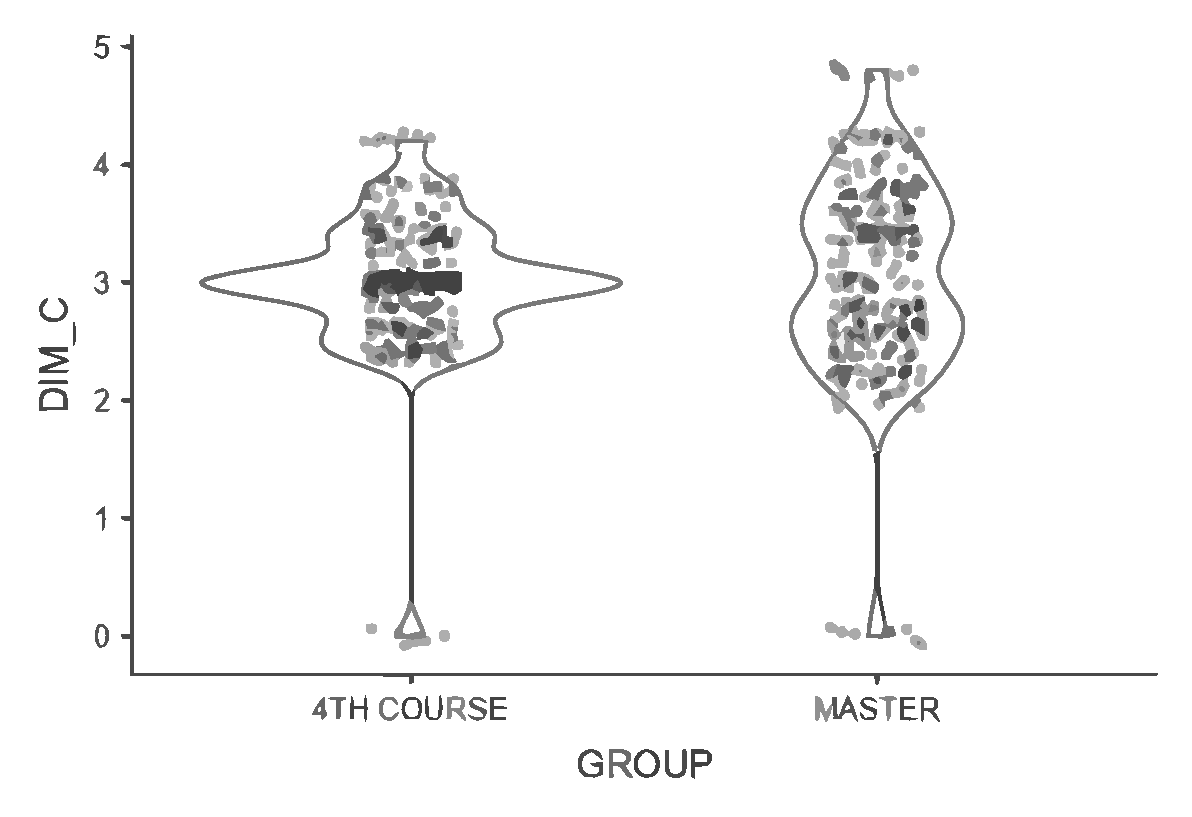
\includegraphics[width=0.65\textwidth]{fig3.pdf}
 \caption{Descriptive data for Dimension C.}
 \label{fig3}
 \source{own elaboration.}
\end{figure}

\Cref{fig3} shows how the subjects’ responses are grouped around the mean, showing indifference in the items that make up this dimension. No differences are observed between the groups surveyed.

Regarding Dimension D (TTE) the respondents give a mean response to the items of 2.76, which shows that they "disagree" with the items.

\begin{figure}[htbp]
 \centering
 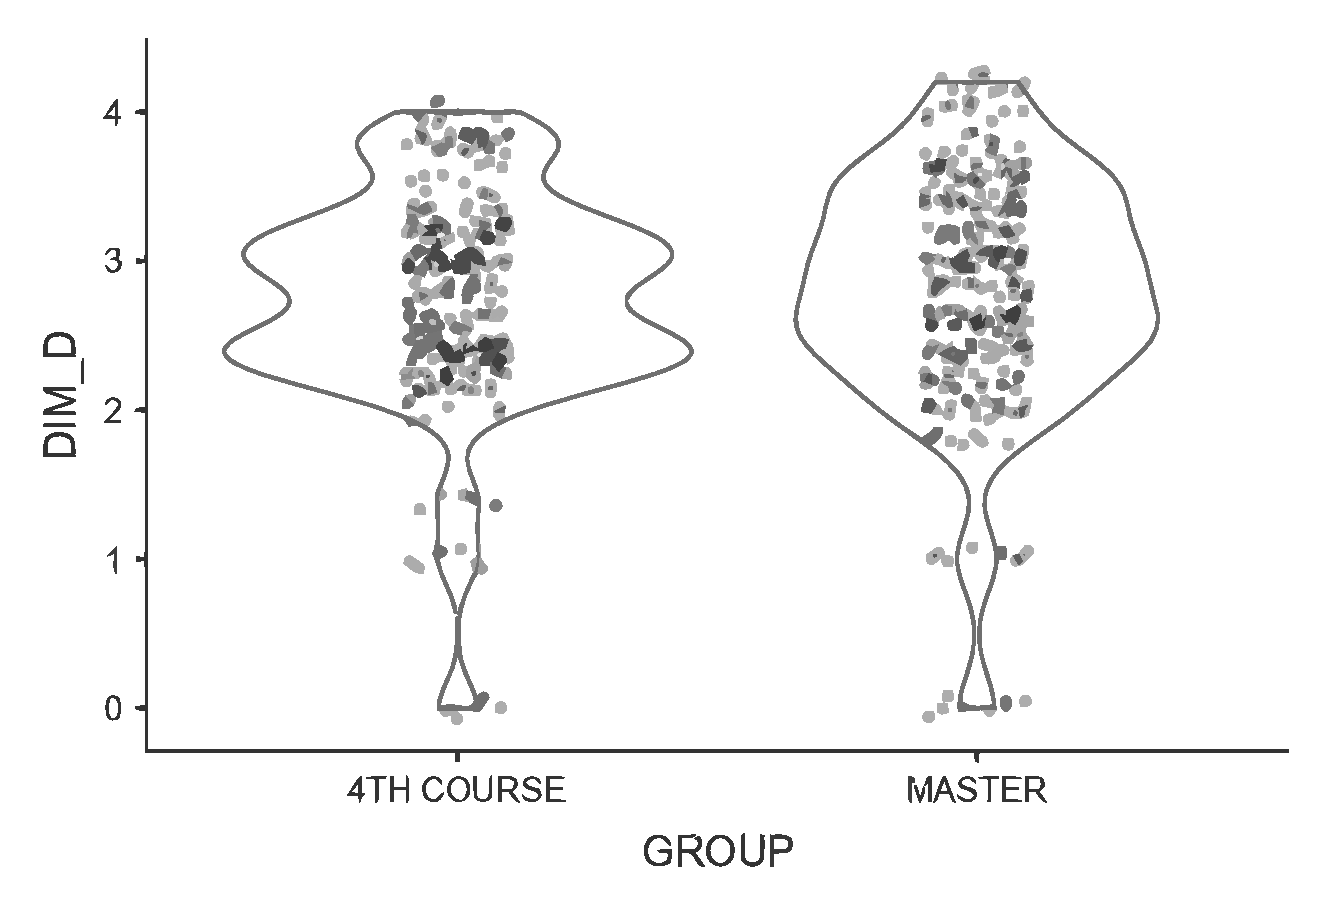
\includegraphics[width=0.65\textwidth]{fig4.pdf}
 \caption{Descriptive data for Dimension D.}
 \label{fig4}
 \source{own elaboration.}
\end{figure}

\Cref{fig4} shows that in relation to ecological teacher training, there is disagreement with the items raised, with no differences between the groups surveyed.

Finally, in Dimension E (TTP), the mean number of responses is 2.76, indicating "disagreement" with the items that make up this dimension.

\begin{figure}[htbp]
 \centering
 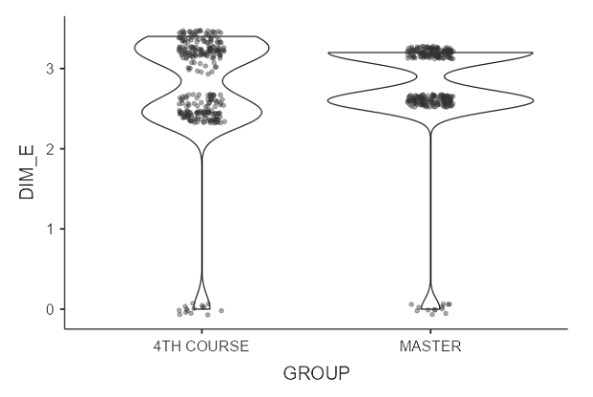
\includegraphics[width=0.65\textwidth]{fig5.png}
 \caption{Descriptive data of the E dimension.}
 \label{fig5}
 \source{own elaboration.}
\end{figure}

\Cref{fig5} shows very little difference between the responses of the two groups to the items that make up the dimension of teacher training in pandemics, being in disagreement with the ideas marked in this dimension.

\subsection{Confirmatory factor analysis (CFA).}
The SEM methodology consists of a series of phases according to \textcite{kaplan2000} %Kaplan (2000) 
and \textcite{kline2005}, %Kline (2005), 
which we will define as four.

Phase I. — Specification of the Measurement Model: the conceptual model of the Likert scale obtained from the exploratory factor analysis is composed of 21 observed variables that are grouped into five dimensions.

Phase II. — Identification. Computational Implementation of the System of Structural Equations: to determine if the model is identified we must calculate the degrees of freedom, in our case the value is 108 gl, so we can say that the model is over identified.

Phase III. — Parameter estimation: the model estimation phase includes a graphical representation of the theoretical-conceptual structure of the instrument under analysis, as shown in \cref{fig6}.

\begin{figure}[htbp]
 \centering
 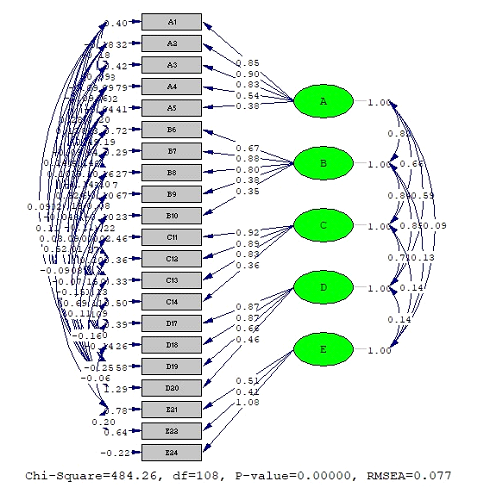
\includegraphics[width=0.85\textwidth]{fig6-2.png}
 \caption{Graphical representation of the natural measurement model of the Likert scale.}
 \label{fig6}
 \source{own elaboration.}
\end{figure}

Figure 6 shows the items, their relationship with the different dimensions, and the regression coefficients of each relationship, which are detailed below.

We reviewed the regression coefficients between the latent and observed variables, the interpretation being as follows:

\begin{itemize}
    \item Dimension A (Teacher training): 
    \\ Greater influence of the latent variable on:
    \\ A2 (.90). - University teacher training is sufficient for my educational practice.
    \\ A1 (.85). - Current teacher training satisfies my training concerns.
    \\ Less influence of the latent variable on:
    \\ A5 (.35). - Teacher training is the key to an educational system in line with the 21st century.
    
    \item Dimension B (Teacher training in inclusive education): 
    \\ Greater influence of the latent variable on:
    \\ B7 (.88). - The inclusive teacher training offered by the university is sufficient for my educational practice.
    \\ B8 (.80). - The inclusive teacher training offered by non-university institutions is sufficient for my educational practice.
    \\ Less influence of the latent variable on:
    \\ B10 (.35). - Inclusive teacher training is the key to an education system in line with the 21st century.
    
    \item Dimension C (Teacher training in technologies):
    \\ Greater influence of the latent variable on:
    \\ C11 (92). - Current technological teacher training satisfies my training concerns.
    \\ C12 (.89). - The technological teacher training offered by the university is sufficient for my educational practice.
    \\ Less influence of the latent variable on:
    \\ C14 (.36). - Technological teacher training offered by foreign institutions is of higher quality than the national one.
    
    \item Dimension D (Teacher training in ecology):
    \\ Greater influence of the latent variable on:
    \\ D17 (.87). - The ecological teacher training offered by the university is sufficient for my educational practice.
    \\ D18 (.87). - The ecological teacher training offered by non-university institutions is sufficient for my educational practice.
    \\ Less influence of the latent variable on:
    \\ D20 (.46). - Ecological teacher training is the key to an educational system in accordance with the 21st century.
    
    \item Dimension E (Teacher training in times of pandemic):
    \\ Greater influence of the latent variable on:
    \\ E24 (1.08). - Ecological teacher training offered by foreign institutions is of higher quality than the national one in times of pandemic.
    \\ Less influence of the latent variable on:
    \\ E22 (.41). - The inclusive teacher training offered by the university is sufficient for my educational practice in times of pandemic.
\end{itemize}

The relationship between the latent variables is given by: A-B (.82), A-C (.66), A-D (.59), A-E (.09), B-C (.84), B-D (.85), B-E (.13), C-D (.71), C-E (.14) and D-E (.14).

The highest ratio is given by: A-B (.82), B-C (.84), B-D (.85) and C-D (.71).

The lowest ratio is given by: A>E (.09), B>E (.13) and D>E (.14).

Phase IV. — Fit assessment: in this stage we use goodness-of-fit indices and criteria to relate the validation evidence to the dimensional structure of the instrument being assessed (Table 5).

\begin{table}[htpb]
\caption{Goodness-of-fit indices.}
\label{tab5}
\centering
\begin{tabular}{p{0.2\textwidth}llllllllll}
\toprule 
& X2 & X2/gl & GFI & RMSEA & ECVI & IFI	& NFI & RFI & AFGI
\\
\midrule
Valor real & p=.000	& 4.28 & .92 & .077 & .79 & .98 & .97 & .96 & .92
\\
Valor ideal & p<5 & <5 & >.90 & <.08 & >valor	& >.95 & >.95 & >.95 & >.90
\\
\bottomrule
\end{tabular}
\source{Prepared by the authors based on \textcite{levy2006}.}
\centering
\end{table}

Table 5 shows the real value and the ideal value, following \textcite{levy2006}, %Levi, Varela and Abad (2006), 
showing that the criteria of all the goodness-of-fit indices are met, so that the model is fully confirmed.

\section{Discussion and conclusions}
The data analysis resulting from the research allows affirming the relationship between the study dimensions, as well as obtaining a reliable, validated and confirmed research instrument to analyze the relationships between the established dimensions, achieving the established general objective, confirming the study hypothesis and demonstrating that we have a relationship between the different elements, Thus, it is very interesting the idea that the ecological training offered by foreign institutions is of higher quality than the national one in times of pandemic, as well as that teacher training is key for an educational system according to the XXI century in times of pandemic, ideas of great value in the constructed scale. The perception that international training is more valuable than national training is still latent in our participants, at least as far as ecology is concerned. On the other hand, whether teacher training in educational inclusion is sufficient or not, is something that worries the surveyed subjects too much, and shows a disturbing reality. On the other hand, the ANOVA carried out shows a strong relationship between the responses of the two participating groups in terms of teacher training in inclusive education and ecology, being lower in the other dimensions (technology, training in pandemic), thus proving the homogeneity of the groups in terms of inclusion and ecology, not so much with the other dimensions. The descriptive analysis is very revealing, as it shows in general "indifference" to the issues raised in terms of inclusive education and education in technologies, being "in disagreement" in terms of teacher training, teacher training in ecology and training in times of pandemic, showing little hope for the future of teacher training in general.

With the exposed, it is possible to glimpse a panorama that should lead us to reflect on the future of teacher training. Despite the limitation of not having included teachers from primary education centers in the sample, with the selected sample it is already possible to detail some very valuable issues, validated by the CFA, thus, teacher training in inclusive education and technologies is something that is taken for granted in the mentality of our subjects, however, it is appreciated the need to include training in ecology, and more in times of pandemic, where the environmental has taken great importance, it is clear that in relation to teacher training, it must meet the demands of the subject; that the training in inclusive, technological and ecological education offered by universities is sufficient for educational practice (at least this is the perception of the subjects surveyed) and, finally, that when speaking of teacher training, it is understood that it will be inclusive, technological and ecological (to this degree of importance) without much influence from the fact that we are in times of pandemic. On the other hand, teacher training in inclusive education should have firstly aspects of ecology and secondly of technology, regardless of whether or not it is under covid19. Teacher training in technology should take into account ecological aspects, with little influence due to the pandemic, and finally, teacher training in ecology has hardly any influence on whether or not it is under covid19. All in all, we conclude that teacher training, which we consider to be inclusive, technological and ecological, must continue its course, whether or not there is a pandemic.

\section{Financement}

Work arising from the project: "Training of University Teachers in ICT to Support Students with Disabilities". Type of Project/Grant: State Plan 2017-2020 Challenges - R+D+i Projects. Referencia: PID2019-108230RB-I00. Included in the Ibero-American Network for the development of the Professional Identity of Teachers (RED RIDIP). of the Teacher (RED RIDIPD) (University of Jaén, Spain)
%%%%%%%%%%%%%%%%%%%%%%%%%%%%%%%%%%%%%%%%%%%%%%%%%%%%%%%%%%%%%%%%%%%%%%%%%%%%%%%%%%%%%%%%%%%%%%%%%%%%%%%%%%%%%%%%%%%%%%%%%%%%%%%%%%%%%%%%%%%%%%%%%%%%%%%%%%%%%%%%%%%%%%%%%%%%%%%%%%%%%%%%%%%%%%%%%%%%%%%%%%%%%%%%%%%%%%%%%%%%%%%%%%%%%%%%%%%%%%%%%%%%%%%%%%%%%%%%%%%%%%%%%%%%%%%%%%%%%%%%%%%%%%%%%%%%%%%%%%%%%%%%%%%%%%%%%%%%%%%%%%%%%%%%%%%%%%%%%%%%%%%%%%%%%%%%%%%%%%%%%%%%%%%%%%%%%%%%%%%%%%%%%%%%%%%%%%%%%%%%%%%%%%%%%%%%%%%%%%%%%%%%%%%%%%%%%%%%%%%%%%%%%%%%%%%%%%%%%%%%%%%%%%%%%%%%%%%%%%%%%%%%%%%%%%%%%%%%%%%%%%%%%%%%%%%%%%%%%%



\printbibliography\label{sec-bib}
% if the text is not in Portuguese, it might be necessary to use the code below instead to print the correct ABNT abbreviations [s.n.], [s.l.] 
%\begin{portuguese}
%\printbibliography[title={Bibliography}]
%\end{portuguese}

\end{document}
